\section{Deterministic Model-Based Agent}

\subsection{Design and Algorithm}

The requirements of the deterministic model-based reflex agent other than its definition is that it can represent state with only 3 bits of memory, which implies up to 8 states\footnote{Without loss of generality, we can use one state variable STATE that takes on integers $[0, 7]$ instead of three explicit state bits STATE1, STATE2 and STATE3 because $0 = 000, 1 = 001, 2 = 010, ..., 7 = 111$.}.

We want the agent to suck every dirt. Since the agent has memory, we are able to perform two ``consecutive'' actions by taking advantage of state information. This will allow the agent to steer into the middle of the world in contrast to the simple memoryless reflex agent, which could only suck dirt near the boundaries of the world.

Therefore, we devised an algorithm that can sweep across the entire room and suck every dirt in 8 states or less. We came up with the following algorithm that sweeps all dirt and returns home in at most 7 states:

\begin{enumerate}
	\item Begin at the home cell.
	\item Go north and suck until it hits the south boundary. 
	\item Go one cell east.
	\item Go south and suck until it hits the south boundary.
	\item Go one cell east.
	\item Repeat steps 2-5 until there is a wall that prevents going one cell east.
	\item Traverse the world boundary until it comes home.
\end{enumerate}

To visualize the process, the algorithm does the sweep pattern across the room in figure \ref{fig:motion}.

\begin{figure}[!t]
	\centering
	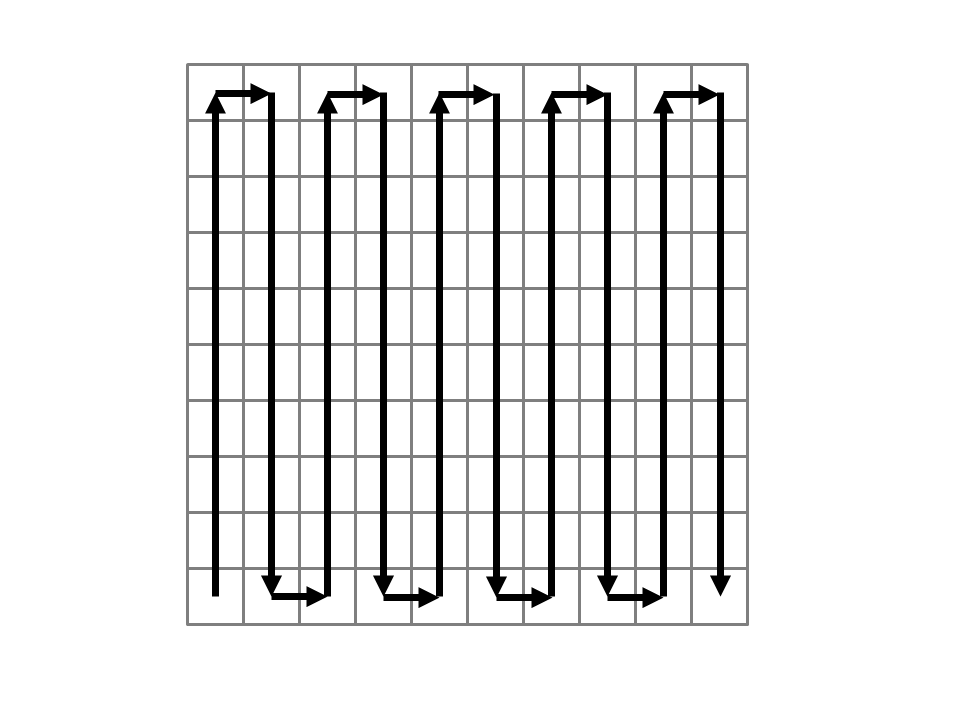
\includegraphics[scale=.30]{img/3-motion.png}
	\caption{The deterministic model-based reflex agent starts at the bottom-left corner and sweeps north, east, south, east, etc. as shown in the figure.}
	\label{fig:motion}
\end{figure}

\subsection{Diagram and Rules}

We can construct the algorithm using 7 states by illustrating the state diagram in figure \ref{fig:states}.

\begin{figure}[!t]
	\centering
	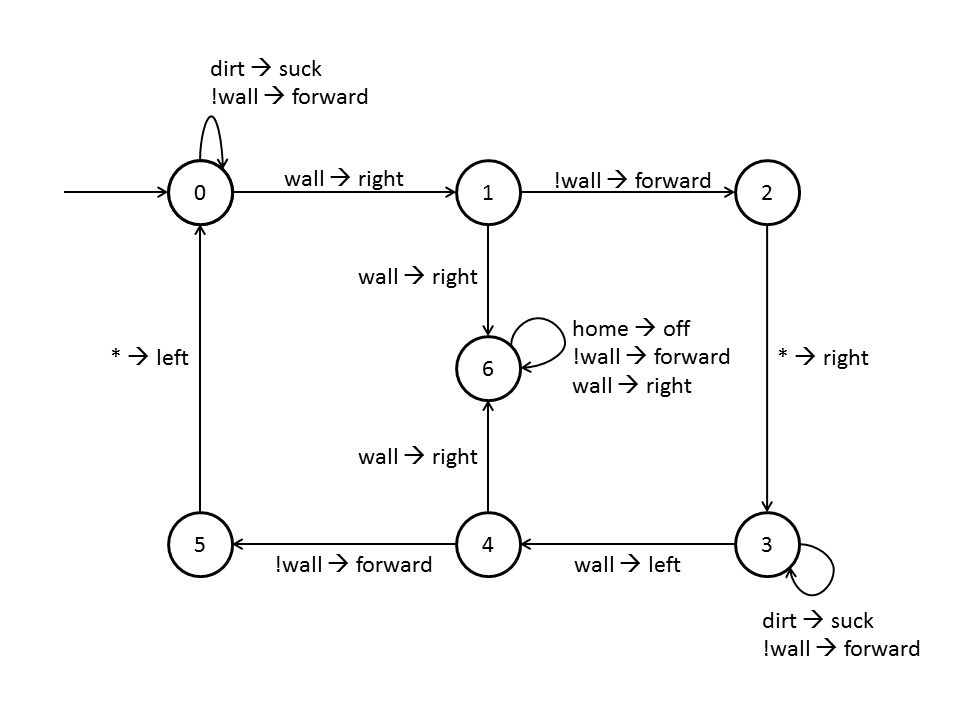
\includegraphics[scale=.30]{img/3-statediag.png}
	\caption{State machine of the model-based reflex agent.}
	\label{fig:states}
\end{figure}

The following is a formal list of if-then rules used to construct the diagram. It is also coded into the agent as the program:

\begin{verbatim}
if STATE=0 and DIRT then SUCK
if STATE=0 and NOT WALL then FORWARD
if STATE=0 and WALL then STATE := 1, RIGHT
if STATE=1 and WALL then STATE := 6, RIGHT
if STATE=1 and NOT WALL then STATE := 2, FORWARD
if STATE=2 then STATE := 3, RIGHT
if STATE=3 and DIRT then SUCK
if STATE=3 and NOT WALL then FORWARD
if STATE=3 and WALL then STATE := 4, LEFT
if STATE=4 and WALL then STATE := 6, RIGHT
if STATE=4 and NOT WALL then STATE := 5, FORWARD
if STATE=5 then STATE := 0, LEFT
if STATE=6 and HOME then OFF
if STATE=6 and NOT WALL then FORWARD
if STATE=6 and WALL then RIGHT
\end{verbatim}

In plain language, state 0 represents a series of reflex actions for sucking and moving north. When the agent hits the top boundary of the world, states 1-2 assist the agent in moving east one square to prepare sucking and moving south. State 3 (symmetric to state 0) represents a series of reflex actions for sucking and moving south. When the agent hits the bottom boundary of the world, states 4-5 (symmetric to states 1-2) assist the agent in moving east one square to prepare sucking and moving north. The cycle repeats until the agent can no longer move east, as detected in states 1 and 4. If that is the case, then the agent moves to state 6, which is a series of reflex actions to navigate the agent around the edges of the map until it reaches home.

Therefore, we have also verified that the state diagram is equivalent to the algorithm.

